
\chapter{Discrete Ordinates Method}
\label{lec:discreteordinates}

In the last two lectures, we dealt exclusively with the integral form of the transport equation and ways to solve it numerically.  Now, we return to the integro-differential form of the equation and introduce the \textit{discrete ordinates ($S_N$) method}, one of the most widely-used deterministic transport methods.  We subsequently introduce the method of \textit{source iteration} for treating the scattering source and finish with a brief overview of acceleration via the methods of coarse mesh rebalance (CMR) and coarse mesh finite difference (CMFD).  As in previous lectures, we provide a simple code that implements some of the concepts discussed.

\section*{A Discrete Angle Domain}

The integral methods of the last two lectures are useful in many applications because they effectively eliminate the angular variable.  If we are to treat the transport equation in its integro-differential form, we need a way to handle the angles.  For the sake of brevity, we limit our discussion to transport in slab geometry with isotropic sources and scattering, for which the transport equation reduces to
\begin{equation}
\begin{split}
 \mu \frac{\partial \psi}{\partial x} + \Sigma_t(x)\psi(x,\mu) &= \frac{\Sigma_s(x)}{2}\int^1_{-1}d\mu' \psi(x,\mu') + \frac{S(x)}{2} \\
                                                               &= \frac{\Sigma_s(x)}{2}\phi(x) + \frac{S(x)}{2} \\
\end{split}
 \label{eq:slabtransportequation}
\end{equation}

The discrete ordinates method consists of requiring Eq. \ref{eq:slabtransportequation} to hold only for discrete values $\mu$.  In other words, we require
\begin{equation}
 \mu_n \frac{\partial \psi}{\partial x} + \Sigma_t(x)\psi(x,\mu_n) = \frac{\Sigma_s(x)}{2} \phi(x) + \frac{S(x)}{2} \, .
 \label{eq:snequation}
\end{equation}
What about $\phi$?  This is where the approximation is actually made.  Because we have $\psi$ only at discrete angles $\mu_n$, we cannot perform the continuous integral.  We do the next best thing and compute a weighted sum:
\begin{equation}
 \phi(x) \approx \sum^N_{n=1} w_n  \psi_n(x) \, ,
 \label{eq:phiquad}
\end{equation}
where we have introduced the notation $\psi_n(x) \equiv \psi(x,\mu_n)$.  

The only actual requirement on $w_n$ is that they satisfy
\begin{equation}
 \sum^N_{n=1} w_n = 2 \, ,
\end{equation}
since this sum represents $\int^1_{-1} d\mu = 2$.  Of course, we don't choose the weights arbitrarily, nor do we choose the cosines $\mu_n$ arbitrarily.  The choice of both is the art of numerical quadrature.

\section*{Intermission: Numerical Quadrature (a.k.a. Numerical Integration)}

You saw application of the \textit{trapezoid rule} in the integral transport code of Lecture \ref{lec:integral}.  You have probably seen the trapezoid rule in previous classes, and if not that, then certainly the even simpler \textit{Riemann sum} approximation to integrals, here in the form of the \textit{midpoint rule}:
\begin{equation}
 \int^b_a f(x)dx \approx  \Delta \sum^{N-1}_{n=0} f \Big ( a + (n+1/2)\Delta \Big ) \, ,
\end{equation}
where
\begin{equation}
 \Delta = \frac{b-a}{N} \, ,
\end{equation}
and $N$ is the number of divisions in the center of which $f$ is evaluated.

The general form of a quadrature rule is
\begin{equation}
 \int^b_a f(x) dx \approx  \sum^{N-1}_{n=0} w_n f(x_n) \, , 
\end{equation}
and we see that the midpoint rule chooses equal weights $w_n = w = \Delta$ and evaluates $f$ at equally spaced points $x_n = a+(n+1/2)\Delta$.  The trapezoid rule also takes evenly spaced points, $x_n = a + n\Delta$, for $n = 0 \ldots N$, and with $w_0 = w_N = 0.5\Delta$, and $w_n = \Delta$, $0 < n < N$.

Other quadrature sets using evenly spaced points also exist.  One general class consists of the \textit{Newton-Cotes formulas}, which interpolate $f(x)$ using various order polynomials and thus allows for analytic integration.  The midpoint rule and the trapezoid rule are the simplest examples, using zeroth order and first order polynomials. Another example is \textit{Simpson's rule}, defined
\begin{equation}
\begin{split}
 \int^b_a f(x) dx \approx & \frac{\Delta}{3} \Big ( f(a)+4f(a+\Delta) +2f(a+2\Delta)+4f(a+3\Delta) \\
                          &  +2f(a+4\Delta)+\ldots+ 4f(b-\Delta) + f(b) \Big ) \, .
\end{split}
\end{equation}
Simpson's rule is based on a piece-wise quadratic interpolation of sets of three points and can often be a very good ``quick and dirty'' way to integrate numerically. The reader is encouraged to consult a numerical analysis text for more details.

In many cases, it is possible to use fewer, non-equally spaced points (with unique weights) to yield accurate integral approximations that would otherwise take many equally spaced points.  One such scheme is Gauss-Legendre quadrature, which is the standard quadrature used to define $\phi$ in Eq. \ref{eq:phiquad}.  The $n$-point Gauss-Legendre scheme is constructed so that polynomials of degree less than or equal to $2n-1$ are integrated exactly over the domain of interest.  

Consider a 2-point Gauss-Legendre scheme, i.e. $\int^{1}_{-1} f(x)dx = w_1 f(x_1) + w_2 f(x_2)$.  We have four unknowns, so we need four equations.  The simplest case is to integrate the monomials $1$, $x$, $x^2$, and $x^3$ over the desired range.  Doing so, we get the set of equations
\begin{equation}
 \begin{split}
   \int^1_{-1} 1   dx = 2           & = w_1 + w_2  \\
   \int^1_{-1} x   dx = 0           & = w_1 x_1 + w_2 x_2  \\
   \int^1_{-1} x^2 dx = \frac{2}{3} & = w_1 x^2_1 + w_2 x^2_2  \\
   \int^1_{-1} x^3 dx = 0           & = w_1 x^3_1 + w_2 x^3_2  \, .
 \end{split}
\end{equation}
This system is solved for $w_1 = w_2 = 1$, $x_1 = -1/\sqrt{3}$, and $x_2 = 1/\sqrt{3}$.  Interestingly, $x_1$ and $x_2$ are the roots of the second-order Legendre polynomial $P_2(x) = x^2 - 1/3$.  In fact, the $x_i$ for any $n$-point Gauss-Legendre scheme are the $n$ roots of the $n$th order Legendre polynomial---hence the name of the quadrature rule\footnote{It should be noted that an entire class of Gaussian quadratures exists based on use of other sets of polynomials to approximate integrals where $f$ is weighted by some weighting function associated with the polynomials.  An important example is the Gauss-Chebyshev quadrature, where we approximate the integral $\int^1_{-1} \frac{f(x)}{\sqrt{1-x^2}}dx$. The $x_i$ are found to be roots of the Chebyshev polynomials.}. The weights are defined
\begin{equation}
 w_i = \frac{2(1-x^2_i)}{(n+1)^2(P_{n+1}(x_i))^2} \, .
\end{equation}
As a reference, the Gauss-Legendre abscissa and weights are given in Table \ref{tbl:gaussquad} for $N=2$, $4$, and $6$.  Note, odd orders are not used because the abscissa would then include $x=0$.  Since our goal is ultimately to integrate over $\mu$, and since we shall encounter terms with $1/\mu$, we simply avoid the singularity by choosing even $N$.

\begin{table}[ht]
 \caption{Gauss-Legendre quadrature parameters.}
 \begin{center} 
 {\small
 \begin{tabular*}{0.50\textwidth}{@{\extracolsep{\fill}} ccc} 
  \toprule 
    $N$   & $\mu_i$ & $w_i$   \\
  \midrule      
    2     &  $\pm 0.5773502691$  &  1  \\
  \midrule 
    4     &  $\pm 0.8611363115$  &  0.3478548451  \\
          &  $\pm 0.3399810435$  &  0.6521451549  \\
  \midrule      
    6     &  $\pm 0.9342695142$  &  0.1713244924  \\
          &  $\pm 0.6612093864$  &  0.3607615730  \\
          &  $\pm 0.2386191860$  &  0.4679139346  \\
  \bottomrule 
 \end{tabular*}
 } 
 \end{center} 
 \label{tbl:gaussquad}  
\end{table}


\section*{A Discrete Spatial Domain}

We next deal with the spatial variable, using the finite volume method.  Consider the discretization of Figure \ref{fig:sndisc}.  The slab is discretized into $I$ regions, each of which is assumed to have constant cross-sections and sources, denoted $\Sigma_{ti}$ and so forth.  The cell centers are given by $x_i$, and the cell edges by $x_{i\pm 1/2}$.  For a slab defined over $0 \leq x \leq L$, $x_{1/2} = 0$ and $x_{I+1/2} = L$.

\begin{figure}[ht] 
    \centering
    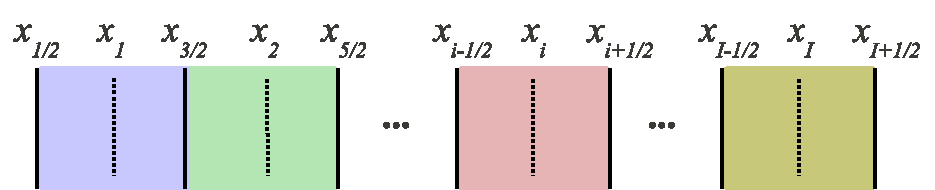
\includegraphics[keepaspectratio, width = 5.0 in]{images/sndisc}
    \caption{Discrete ordinates spatial discretization.}
    \label{fig:sndisc}
\end{figure}

Now, we integrate Eq. \ref{eq:snequation} over cell $i$:
\begin{equation}
  \int^{x_{i+\frac{1}{2}}}_{x_{i-\frac{1}{2}}} dx \Big ( \mu_n \frac{\partial \psi_n}{\partial x} + \Sigma_t(x)\psi_n(x) \Big ) =  \int^{x_{i+\frac{1}{2}}}_{x_{i-\frac{1}{2}}} dx  \Big ( \frac{\Sigma_s(x)}{2} \phi(x) + \frac{S(x)}{2} \Big ) \, ,
\end{equation}
so that
\begin{equation}
   \mu_n ( \psi_{i+\frac{1}{2},n} - \psi_{i-\frac{1}{2},n} ) + \Delta_i \Sigma_{ti}\psi_{i,n} =  \frac{\Delta_i}{2} \Big ( \Sigma_{is} \phi_i +  S_i \Big ) \, ,
\end{equation}
where $\Delta_i \equiv x_{i+\frac{1}{2}} - x_{i-\frac{1}{2}}$ and where the integrals have been approximated via the midpoint rule where needed.  For the sake of brevity, we switch to the emission density, defining
\begin{equation}
 Q_i =  (\Sigma_{is} \phi_i +  S_i)/2 \, ,
\end{equation}
so that
\begin{equation}
   \mu_n ( \psi_{i+\frac{1}{2},n} - \psi_{i-\frac{1}{2},n} ) + \Delta_i \Sigma_{ti}\psi_{i,n} =  \Delta_i Q_i \, .
   \label{eq:discsneq}
\end{equation}

Eq. \ref{eq:discsneq} is a good first step, but we're not done.  Imagine we know the angular flux entering the left side of slab $i$.  We would like to be able to compute the angular flux leaving $i$ to the right.  Doing exactly this over the entire domain is referred to as ``sweeping'' and is a common technique for hyperbolic problems, as it allows us to propagate boundary conditions along the direction of neutron paths.  The problem with Eq. \ref{eq:discsneq} is that we have another unknown: $\psi_{i,n}$, the cell-centered angular flux.  There are several approximations we can use, and we develop two: the diamond difference (DD) and step difference (SD) methods.

For both DD and SD, we define the cell-centered angular flux by
\begin{equation}
 \psi_{i,n} = \frac{1+\alpha_n}{2} \psi_{i+\frac{1}{2},n} + \frac{1-\alpha_n}{2} \psi_{i-\frac{1}{2},n}  \, ,
 \label{eq:ccpsi}
\end{equation}
where
\begin{equation}
 \alpha_n =
 \begin{cases} 0             &   \text{for DD}  \\
               |\mu_n|/\mu_n &   \text{for SD}  \\
 \end{cases} \, .
 \label{eq:alpha}
\end{equation}

The DD method is probably the most ubiquitous of the simple schemes available.  It essentially says the angular flux varies linearly within a cell, and it provides second-order accuracy.  Unfortunately, the DD method can lead to negative fluxes for $\Delta_i$ too large, demonstration of which is left as an exercise.  On the other hand, the SD method cannot yield negative fluxes, but is only first-order accurate.  For the SD method, note that the cell-center angular flux is equal to the incident angular flux at the edge.

\section*{Sweeping Formulas}

We hinted above that we can solve the discrete ordinates equations via use of sweeps across the domain.  In slab geometry, this consists of sweeps to the right for $\mu_n > 0$ and sweeps left for $\mu_n < 0$.  If we have vacuum or some other known boundary flux, we start with that condition, as reflective conditions require information from a sweep having come from the opposite direction.  If all conditions are reflective, a guess must be made for one, which will likely increase the number of iterations required (we'll get to iterations below).

Substituting Eq. \ref{eq:ccpsi} into Eq. \ref{eq:discsneq} and rearranging, we find for sweeping right
\begin{equation}
 \psi_{i+\frac{1}{2},n} = A^+_{i,n} \psi_{i-\frac{1}{2},n} + B^+_{i,n} Q_i \, ,
 \label{eq:rightsweep}
\end{equation}
and sweeping left
\begin{equation}
 \psi_{i-\frac{1}{2},n} = A^-_{i,n} \psi_{i+\frac{1}{2},n} + B^-_{i,n} Q_i \, , 
 \label{eq:leftsweep}
\end{equation}
where
\begin{equation}
 A^{\pm}_{i,n} = \frac{2\mu_n \mp (1 \mp \alpha_m)\Sigma_{ti}\Delta_i}{2\mu_n \pm (1 \pm \alpha_m)\Sigma_{ti}\Delta_i} \, , 
 \label{eq:Aconstant}
\end{equation}
and
\begin{equation}
 B^{\pm}_{i,n} = \frac{\pm 2 \Delta_i}{2\mu_n \pm (1 \pm \alpha_m)\Sigma_{ti}\Delta_i} \, .
 \label{eq:Bconstant}
\end{equation}

\section*{Source Iteration}

When we introduce scattering into the emission density, the right hand side becomes dependent on the solution.  A common way around this is the so-called source iteration method.  The source iteration method is related to the Neumann iteration scheme discussed in Lecture \ref{lec:integral}, and a connection between the two is left as an exercise.  

Source iteration is characterized by a right hand side that lags behind the left hand side.  More explicitly, we solve the equation
\begin{equation}
   \mu_n ( \psi^m_{i+\frac{1}{2},n} - \psi^m_{i-\frac{1}{2},n} ) + \Delta_i \Sigma_{ti}\psi^m_{i,n} =  \Delta_i Q^{m-1}_i \, ,
   \label{eq:discsneqsi}
\end{equation}
where $m$ is the iteration index and 
\begin{equation}
 Q^{m-1} = \frac{1}{2} (\Sigma_{is} \phi^{m-1}_i +  S_i) \, .
\end{equation}
For $m=1$, we need $q^0$.  Often, $\phi^0$ is simply set to zero, unless a better initial guess is easily made.  

The iterations continue until the updated fluxes change insignificantly.  This is usually quantified in a relative sense for the scalar flux by
\begin{equation}
 \frac{ \max | \phi^{m}-\phi^{m-1} |}{\phi^{m-1}}  < \epsilon_{\phi} \, 
 \label{eq:siconvergence}
\end{equation}
for some small $\epsilon_{\phi}$.

\section*{Acceleration}

The discrete ordinates method is in theory a very fast, memory-efficient technique.  Unless the angular flux is needed explicitly, only one set of edge angular fluxes is needed at a time (e.g. the left edge flux for computing the right edge flux, which then can overwrite the left edge flux).  

Despite the algorithmic simplicity of the method, the underlying source iteration scheme can be obnoxiously slow for problems with high scattering ratios.  Several methods have been introduced over the years to accelerate the source convergence.  Of these, diffusion synthetic acceleration (DSA) is probably the most powerful and widespread.  The method essentially involves performing a diffusion solve to update the scalar flux, and has shown spectacular success for a wide variety of problems.  However, DSA can be difficult if not impossible to implement for certain geometries and/or discretization schemes, as it requires a very strict consistency between the transport and diffusion mesh. Instead, we look at two other relatively simple methods that have been quite successful: the \textit{coarse mesh rebalance} (CMR) and \textit{coarse mesh finite difference} (CMFD) methods.

\section*{Coarse Mesh Rebalance}

CMR was probably the first wide-spread method for acceleration discrete ordinates calculations.  Its foundation rests in the \textit{neutron balance equation}, which we obtain in 1-d by integrating Eq. \ref{eq:slabtransportequation} over angle, yielding
\begin{equation}
\begin{split}
 \frac{\partial }{\partial x}J(x) + \Sigma_t(x) \phi(x) = \Sigma_{s}(x)\phi(x) + S(x) \, ,
\end{split}
\label{eq:balance}
\end{equation}
where $J = \mathbf{J}\cdot \hat{i}$ is the net current in the $x$ direction. Now suppose we divide the domain into a number of coarse meshes, indexed by $j$, with cell edges at $x_{j-\frac{1}{2}}$ and $x_{j+\frac{1}{2}}$.  Subtracting the scattering source from both sides and integrating over the $j$th coarse mesh, we obtain
\begin{equation}
\begin{split}
 J_{j+\frac{1}{2}} - J_{j-\frac{1}{2}}  + \int_{x_i} \Sigma_r(x) \phi(x) dx = \int_{x_i} S(x) dx \, .
\end{split}
\end{equation}
Expressing Eq. \ref{eq:net2partial} as $J = J^+ - J^-$, where $+$ indicates to the right and $-$ to the left, we have
\begin{equation}
\begin{split}
 J^+_{j+\frac{1}{2}}- J^-_{j+\frac{1}{2}} - J^+_{j-\frac{1}{2}} + J^-_{j-\frac{1}{2}} + R_j = S_j \, ,
\end{split}
\label{eq:cmrbalance}
\end{equation}
where the partial currents are defined
\begin{equation}
 J^{\pm}_{j+\frac{1}{2}} = \sum_{\mu_n \gtrless 0} \mu_n \psi_{j+\frac{1}{2},n} \, ,
\end{equation}
$R_j$ is the coarse mesh-integrated removal rate, and $S_j$ is the coarse mesh-integrated source.  

Eq. \ref{eq:cmrbalance} must be satisfied by a fully converged fine mesh solution.  For an unconverged iterate, which we denote $\psi^{m+\frac{1}{2}}$, Eq. \ref{eq:cmrbalance} is generally not satisfied.  To force the flux to satisfy neutron balance, we introduce multiplicative rebalance factors $f_j$ such that
\begin{equation}
 \psi^{m+1}_{i,n} =
 \begin{cases} f_j \psi^{m+\frac{1}{2}}_{i,n}     &   x_{j-\frac{1}{2}} < x_{i} < x_{j+\frac{1}{2}} \\
               f_{j-1} \psi^{m+\frac{1}{2}}_{i,n} &   x_{i} = x_{j+\frac{1}{2}} \text{ and } \mu_n > 0 \\
               f_{j+1} \psi^{m+\frac{1}{2}}_{i,n} &   x_{i} = x_{j+\frac{1}{2}} \text{ and } \mu_n < 0 \\
 \end{cases} \, .
 \label{eq:alpha}
\end{equation}
Note the appropriate factor's index denotes from which coarse mesh the neutrons originate. For the case of vacuum boundaries, the corresponding incident partial current vanishes.  For a reflective boundary at the left, $f_0 = f_1$, and similarly for the right boundary.

To illustrate the method, consider a slab with vacuum boundaries divided into three coarse meshes.  Substituting the modified fluxes into the balance equation yields a set of three equations:
\begin{equation}
\begin{split}
  f_1 J^+_{3/2}  - f_2 J^{-}_{3/2}                   + f_1 J^{-}_{1/2} + f_1 R_1 &= f_1 S_1 \\
  f_2 J^+_{5/2}  - f_3 J^{-}_{5/2} - f_1 J^{+}_{3/2} + f_2 J^{-}_{3/2} + f_2 R_2 &= f_2 S_2 \\
  f_3 J^+_{7/2}                    - f_2 J^{+}_{5/2} + f_3 J^{-}_{5/2} + f_3 R_3 &= f_3 S_3 \, ,
\end{split}
\end{equation}
which yields a tridiagonal system written in condensed form as
\begin{equation}
 \mathbf{A} \mathbf{f} = \mathbf{S} \, .
\end{equation}
Solving this equation for $\mathbf{f}$ and updating to $\psi^{m+1}$ allows us to recompute the scattering source, which---hopefully---converges faster than without the rebalancing scheme.  Look to the Further Reading section for references that investigate stability of coarse mesh rebalance.  Algorithm \ref{alg:accel} shows how CMR (or any low order acceleration scheme) can be used within source iteration.

\begin{algorithm}
 \label{alg:accel}
 \caption{Accelerated Source Iteration}
  initialization\;
  \While{$\psi^m$ or $\phi^m$ not converged}{
    compute scattering source \;
    $\psi^{m+\frac{1}{2}} \leftarrow \text{sweep}(\psi^{m})$ \;
    \eIf{using CMR}{
      $\psi^{m+1} \leftarrow \text{cmr}(\psi^{m+\frac{1}{2}})$ \;
    }{
      $\psi^{m+1} \leftarrow \psi^{m+\frac{1}{2}}$ \;
    }
  }
\end{algorithm}



\section*{Coarse Mesh Finite Difference}

The coarse mesh finite difference method has its origins in a nonlinear acceleration technique developed by K. Smith that makes use of discontinuity factors.  With discontinuity factors, any region-integrated high order solution (e.g. from fine mesh transport) can be represented by a low order method (e.g. coarse mesh diffusion).  CMFD makes use of this idea to represent partially converged high order solutions in low order form, followed by subsequent iterations in the low order domain.  This approach is a physical analog of multigrid methods, and its main effect is to dampen low order errors.  What this means is that the high order method will quickly get the ``shape'' right, and a low order acceleration will quickly get the ``magnitude'' right.

We sketch the implementation.  Given a partially converged fine mesh solution, homogenized diffusion coefficients and cross-sections are found for each coarse mesh, as are volume-averaged sources and fluxes.  A coarse mesh diffusion equation is to be solved, but due to an incompletely converged fine mesh solution, discontinuity factors---additive corrections to the effective diffusion coefficients---must be computed to enforce net current continuity between coarse meshes. Once these are defined, the coarse mesh diffusion equations can be solved.  The ratio of the updated average flux to the original average flux of a coarse mesh is used to scale the original fine mesh solution.  The interested student should see the references and exercises for further details.

%  For edge $j+\frac{1}{2}$ joining meshes $j$ and $j+1$, we compute from the high order solution the net current $J_{j+\frac{1}{2}}$ and enforce
% \begin{equation}
%  J_{j+\frac{1}{2}} = -\tilde{D}_{1+\frac{1}{2}} \Big ( \bar{\phi}_{j+1}-\bar{\phi}_{j} \Big ) -\hat{D}_{1+\frac{1}{2}} \Big ( \bar{\phi}_{j+1}-\bar{\phi}_{j} \Big ) \, ,
% \end{equation}
% where
% \begin{equation}
%  \D
% \end{equation}

\section*{A Simple Code}

Here, we provide a simple discrete ordinates code for computing the angular and scalar flux in a slab, given in Listing \ref{list:sn}.  The input requires region (coarse mesh) edge locations, within which the number of fine meshes are defined.  Each region is assigned a material index and volumetric source strength.  The total and scattering cross-sections represent values for different materials; each material can be placed in a region using the appropriate index.  This quick input format allows one to investigate fairly easily a wide range of slab compositions.

Currently, the code is limited to the DD and $S_4$ approximations and vacuum boundaries.  Convergence is tested for $\phi$ only.  The code returns the mesh-centered scalar flux and mesh-edge angular flux.  Within the solver, the notation follows the lecture notation relatively closely.

\lstset{language=Octave,caption=Solution of Slab Problem via Sn, label=list:sn, morecomment=[l]{\%}}
\lstinputlisting{code/sn.m}

% References
\section*{Further Reading}

A good introduction to the discrete ordinates method in 1-d can be found in Chapter 3 in Lewis and Miller \cite{lewis1993cmn}; higher dimensions are covered in Chapter 4 of the same work.  The foundation of the method is usually credited to Chandrasekhar (in the context of stellar radiation) and can be found in his monograph \cite{chandrasekhar1950rt}.  

A review paper by Adams and Larsen \cite{adams2002fim} provides a survey of the many acceleration techniques available for the discrete ordinates equations, and with its several hundred references, is the place to look for further information.  Lewis and Miller provides more information on coarse mesh rebalance, and Cefus and Larsen have assessed its stability \cite{cefus1990sac}.  Park and Cho \cite{park2004cma} have suggested angular-dependent rebalance schemes, and their work is a good place to start to find references to other CMR variations.  The discontinuity factors used in CMFD were first proposed by Smith in the context of homogenization \cite{smith1980shm}, and he later proposed their use for acceleration \cite{smith1983nms}. A recent paper by Zhong et al. \cite{zhong2008itl} provides a modern overview and advanced use of the approach along with a relatively detailed set of equations for implementation.  

Recent advances in the discrete ordinates method include employing advanced Krylov subspace methods, outlined by Warsa, Wareing, and Morel \cite{warsa2004kim}, variations of which are implemented in the state-of-the-art code Denovo \cite{evans2010dnt}.  Moreover, the discrete ordinates equations can be parallelized; the most popular approach is that of Koch, Baker, and Alcouffe \cite{koch1992sfo} (also implemented in Denovo).

For more information on numerical quadrature, see any number of numerical analysis books.  Also, MIT course 18.335 is also highly recommended, as it covers numerical quadrature and many other aspects of numerical methods (including a heavy focus on numerical linear algebra).

\begin{exercises}

  \item \textbf{Negative fluxes}. Using the DD method, express the sweeping step relation in the form
  \begin{equation*}
    \psi_{3/2,n} = A \psi_{1/2,n} + B \, ,
  \end{equation*}
  where $\mu_n > 0$ and $A$ and $B$ are constants to be determined, and eliminate any $\alpha$ terms.  Under what conditions can $\psi_{3/2,n}$ be negative?  Under what conditions, if any, can $\phi_{1,n}$ be negative?  While negative fluxes are not inherently bad numerically, they don't make much physical sense.  Suggest a method for ``fixing'' negative fluxes.

  \item \textbf{Step Difference}.  Implement the step difference method.\footnote{Note, in this and other exercises you are asked to use or modify the given $S_N$ code.  It is also acceptable to use your own code, either written from scratch or via modification of the one given.}

  \item \textbf{Step Characteristic}.  The step characteristic (SC) scheme is another differencing approach based on analytical integration of the transport equation over the fine mesh cell, yielding for example
  \begin{equation*}
    \psi_{i+\frac{1}{2},n}  =  \psi_{i-\frac{1}{2},n} e^{- \frac{\Delta_i \Sigma_{ti}}{\mu}} + \frac{Q_i}{2\Sigma_{ti}} \Big ( 1-e^{-\frac{\Delta_i \Sigma_{ti}}{\mu}} \Big ) \, .
  \end{equation*}
  \begin{enumerate}[(a)]
    \item Derive an expression for $\alpha_{mi}$ as in Eq. \ref{eq:alpha} for use with the SC method.  Note that $\alpha$ in this case is also indexed by the fine mesh index $i$. 
    \item Implement the SC method.
  \end{enumerate}
 
  \item \textbf{Accuracy}.  Here, we want to investigate the accuracy of various difference methods.  To do so, we will use a known analytical solution for as a reference.  See e.g. Appendix A of LeVeque \cite{leveque2007fdm} for more on error analysis.
  \begin{enumerate}[(a)]
    \item Using the $S_6$ approximation, solve \textit{analytically} the discrete ordinates equations for the sample slab problem of Lecture \ref{lec:analytical}.  Implement this reference solution as a function in MATLAB (or your language of choice), so that $\phi(x)$ can be evaluated for any value of $x$.        
    \item Using the DD approximation, solve the $S_6$ equations using 10, 20, 40, 80, and 160, and 320 meshes.  For each case, compute the absolute value of the maximum error between the DD and analytical solution for $\phi$, i.e. find 
    \begin{equation*}
     e^{\text{DD}}_I = \max_{1\leq i \leq I} \Big|\phi^{\text{DD}}_{i}-\phi_{i}^{\text{ref}} \Big |  \, .
    \end{equation*}
    \item Do the same for the SD method.
    \item We say a method is $p$th order accurate if $e(\Delta) \propto \Delta^p$.  Estimate $p$ for both methods. 
    \item Plot the errors for both methods as a function of $\Delta$.  Include also the functions $a\Delta^1$ and $b\Delta^2$, where $a$ and $b$ are constants chosen to yield a nice plot.  Hint: use a log-log plot.
   \end{enumerate}

  \item \textbf{Accuracy: Part Deux}.  Here, we want to investigate the accuracy of the Gauss-Legendre quadrature and hence $S_N$ order.  
  \begin{enumerate}[(a)]
    \item Compute $\phi(x)$ analytically for the sample slab problem of Lecture \ref{lec:analytical}, and make this available as a function.
    \item Compute $\phi$ analytically using the $S_N$ method for orders 2, 4, 8, 16, 32, and 64.  You will have to look up the quadrature parameters for $N > 4$.  
    \item Compute the errors in $\phi$ as in the last problem for $x = 5.0$ and plot as a function of $N$.  
    \item Estimate the ``$p$'' value as in the last problem and comment.  
   \end{enumerate}


  \item \textbf{Reflective Conditions}. Modify the given $S_N$ code to handle reflective conditions, and solve the following problems...

  \item \textbf{CMR}.  Implement CMR in the given $S_N$ code.  Test it on the following problems, using a variety of coarse mesh sizes...

  \item \textbf{CMFD}.  Read the paper by Zhong et al. \cite{zhong2008itl} and derive the CMFD equations in 1-d.  Implement the method in the $S_N$ code and compare it to CMR for the slab configuration given in the last problem.

  \item \textbf{Discrete Ordinates Matrix}.  The discrete ordinates equations are simply a set of coupled differential equations discretized in space and angle.  Consequently, we can express the equations in matrix form.  Consider a uniform slab ($\Sigma_t$ and $\Sigma_s$) with a uniform isotropic source of volumetric strength $S$. Suppose we discretize this slab into three cells of equal width $\Delta$.  Using an $S_2$ approximation with the DD method, and assuming vacuum conditions:
  \begin{enumerate}[(a)]
    \item Cast the sweep-based source iteration scheme in matrix form, expressing the right hand vector in terms of $Q$, the emission density.         
    \item Reformulate the equations so that the source term is brought to the left hand side, thus enabling a direct solution of the equations without source iteration.  
   \end{enumerate}
  For $\Sigma_t = 1.0$, $\Sigma_s = 0.5$, $\Delta = 1.0$, and $S = 1.0$, verify your expressions from parts (a) and (b).  For more on part (b), see the paper by Patton and Holloway \cite{patton2002apg}.

\end{exercises}
